\section{Methods}

We manually designed strategies that organisms could use to cooperate to experimentally demonstrate that the DISHTINY platform selects for detectable hierarchical transitions of individuality.

\subsection{DISHTINY}

\begin{figure*}[t]
\begin{center}
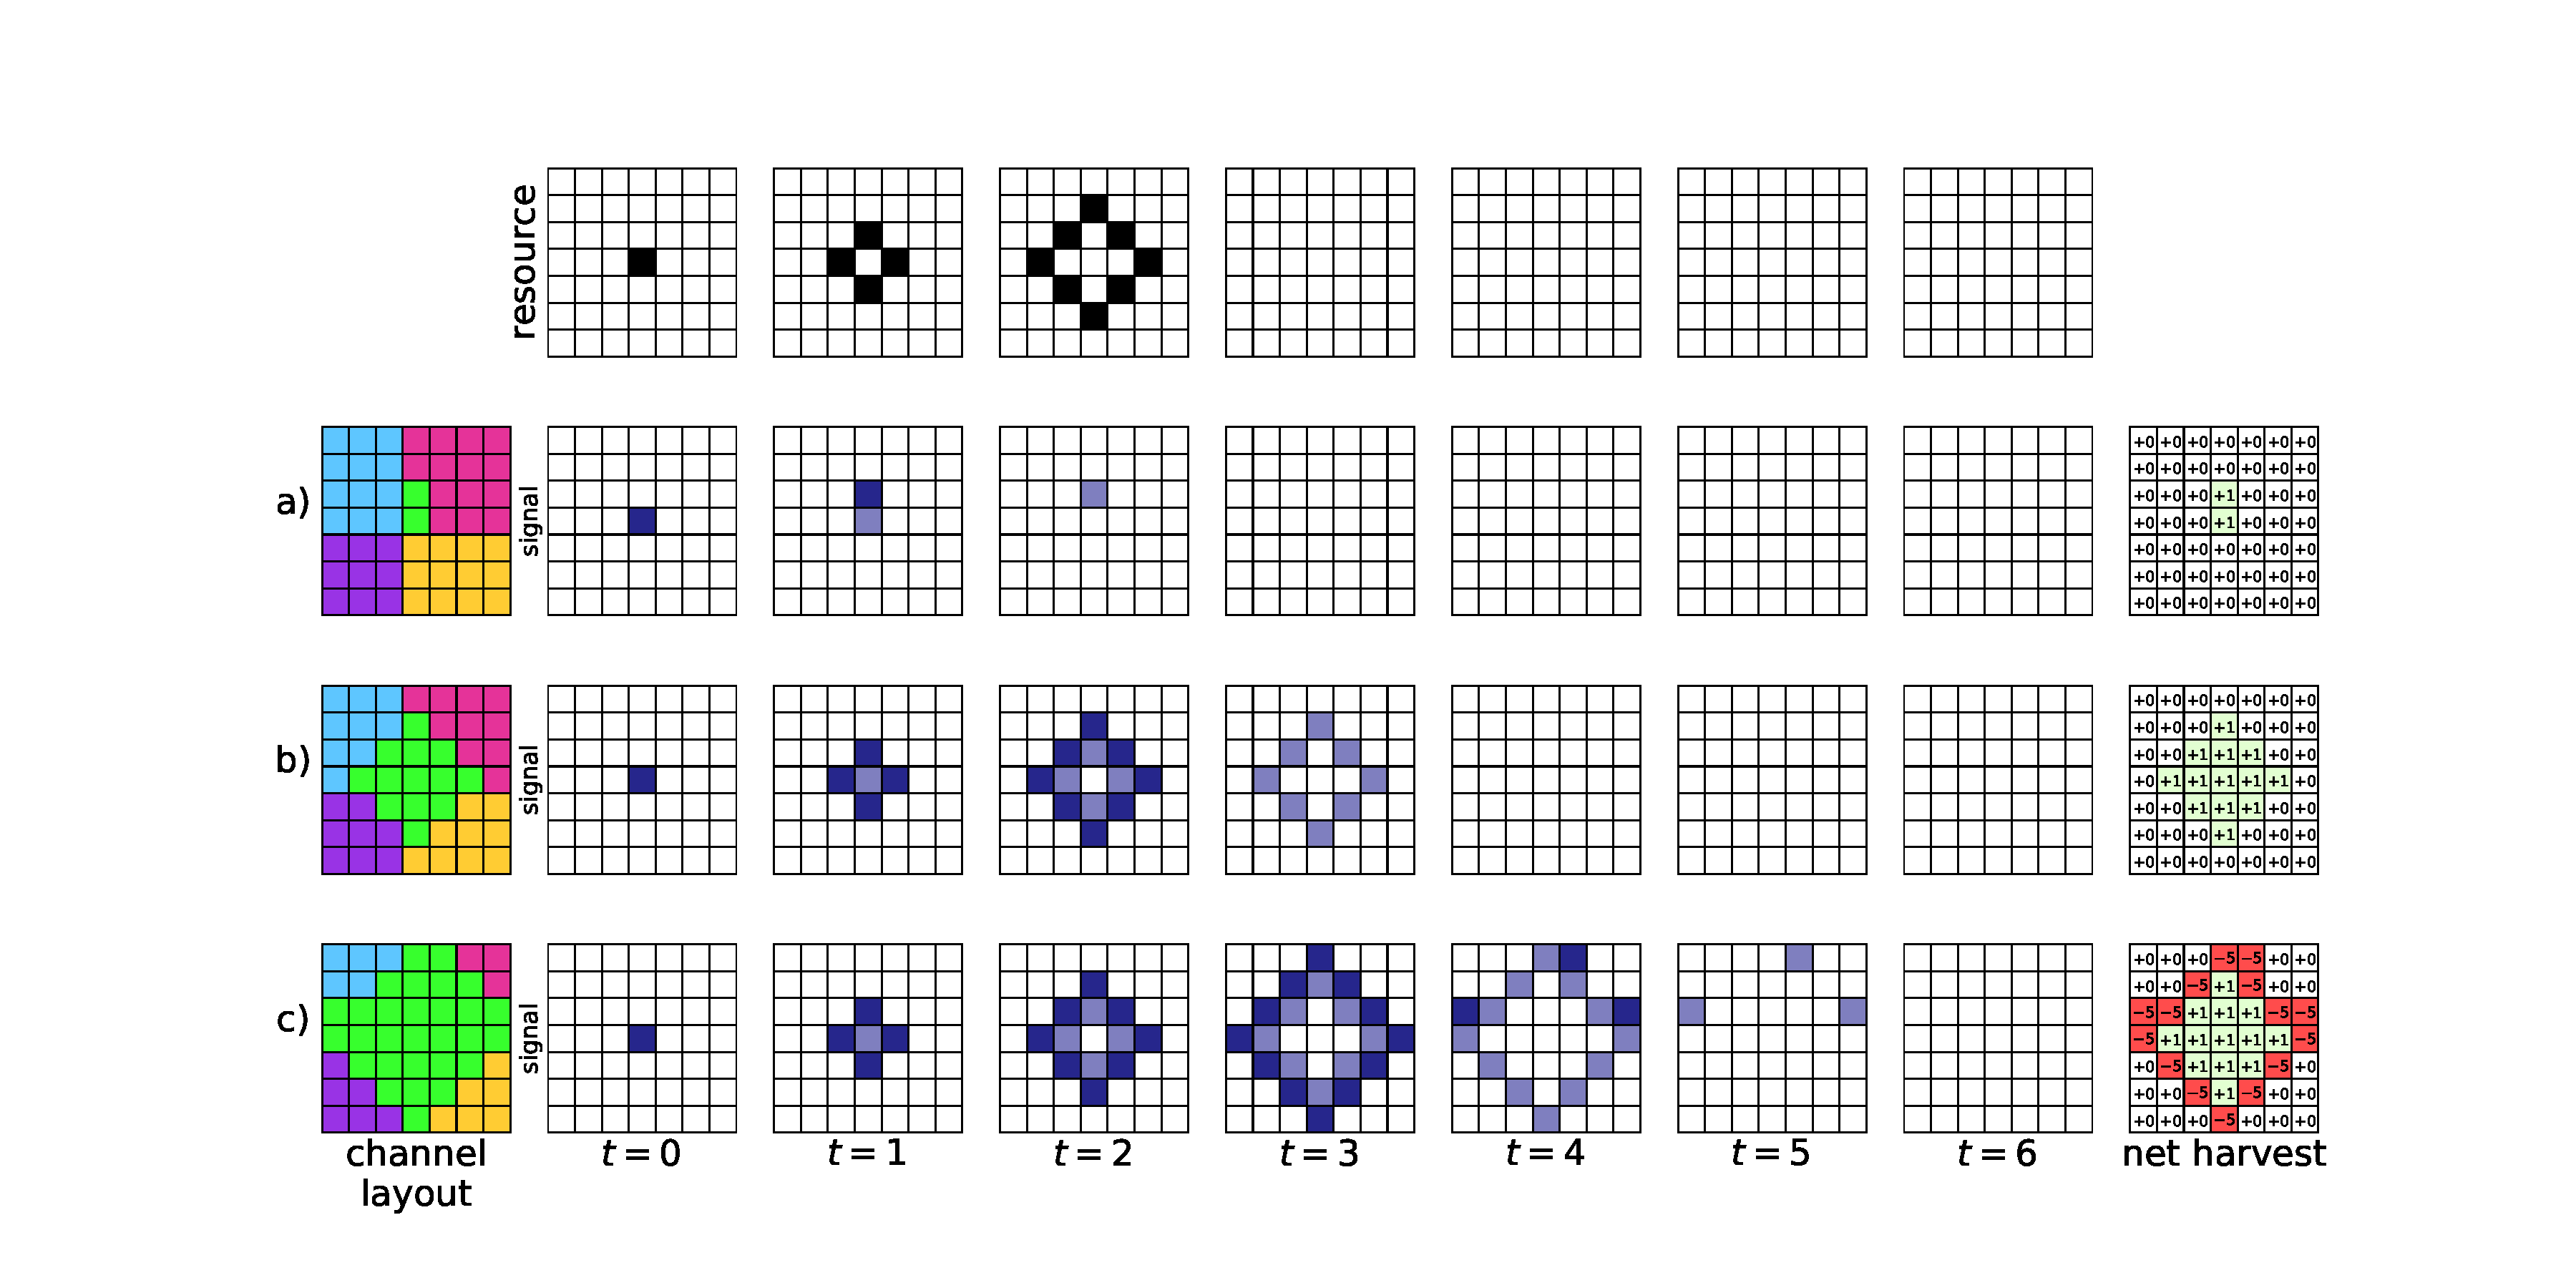
\includegraphics[width=2.0\columnwidth]{img/explanatory}
\caption{
\textbf{Activation signaling, and net resource collection for three different channel configurations during a resource wave event.}
At the top, a resource wave is depicted propagating over three updates and then ceasing for four updates (left to right).
In row $a$, a small channel-signaling group (far left, in green) is activated; tracking the resource wave (top) yields a small net resource harvest (far right).
In row $b$, an intermediate-sized channel-signaling group yields a high net resource harvest.
Finally, in row $c$, a large channel-signaling group incurs a net negative resource harvest.
In rows $a$, $b$, and $c$, dark purple indicates the active state, light purple indicates the quiescent state, and white indicates the ready state.
}
\label{fig:explanatory}
\end{center}
\end{figure*}


We will begin by discussing the implementation of our artificial environment at a single hierarchical level, then lay out how the system scales to multiple levels.

A single continuous-valued resource is tracked.
When organisms accrue sufficient resource, they may choose to pay a cost of $-8$ to reproduce.
As shown Figure \ref{fig:explanatory}, resource is distributed in waves that emanate from a single point.
With each simulation update, the resource wave advances one grid tile outward until it reaches a predefined extent.
The resource wave then ceases.
Coincident with the inception of each resource wave, an activation-quiescence signal wave is triggered at the wave's center point.
Example signal waves are shown in Figure \ref{fig:explanatory}.
With every update, the signal wave passes to adjoining cells registered to the same channel as the cell it emanates from.
The signal wave is not propagated to any cells on any other channel.
In this way, cells sharing the channel of the cell where the resource wave originated are activated coincident with the resource wave.

In order to obtain resource, a cell must be activated by a signal wave as the resource wave passes over.
The cell at the center of a resource wave will always be activated and absorb resource.
However, immediately adjacent cells can only obtain resource by the action of the signal wave --- by sharing the channel of the originating cell.
Cells further off depend on a continuous path of cells extending from the originating cell that signal on the originating channel in order to obtain resource.
As shown in Example $a$ of Figure \ref{fig:explanatory}, the rate of resource collection is determined by the size of a channel signaling network; small or fragmented channel networks will tend to frequently miss out on resource as it passes over.

Importantly, a significant activation cost is paid by each cell that is activated by a signal wave.
This activation cost is outweighed by the amount of resource collected --- cells that activate in concert with a resource wave take away a net benefit.
Recall, though, that resource waves have a limited extent.
Cells that activate outside of the extent of the resource wave or activate out of sync with the resource wave (i.e. are not connected via a direct path to the originating cell) pay a cost.
Cells that frequently activate erroneously bankrupt and die.
In our implementation, organisms that accrue a resource debt of $-11$ or greater are killed.
This scenario is depicted in Example $c$ of Figure \ref{fig:explanatory}.

In this manner, ``Goldilocks'' --- not to small and not too big --- same-channel signaling networks are selected for.
In our implementation, resource waves are seeded at a single location drawn  with uniform probability from the toroidal grid.
Based on this location, resource wave seeds are tiled over the toroidal grid so as to have kissing --- but not overlapping --- extents.
All the waves are updated to completion in synchrony.
Then, another batch of resource waves is seeded.
This process ensures that selection for ``Goldilocks'' same-channel signaling networks is uniformly distributed over the toroidal grid.

Organisms may control the size and shape of their same-channel signaling group by strategic control of reproduction.
Three choices are afforded: whether to reproduce at all, where among the four adjoining tiles of the toroidal grid to place their offspring, and whether the offspring should be registered to the parent's signaling channel or should instead be registered to a randomly chosen signaling channel.
New channels IDs are drawn uniformly from the integer range 1-4194303.
No guarantees are made about the uniqueness of an offspring's channel ID with respect to the channel IDs of the parent or other neighboring cells.

Hierarchical levels are introduced into the system through multiple instantiations of this resource wave/channel-signaling wave scheme.
In our experiments, we worked with two resource wave/channel-signaling levels.
We refer to them as level zero and level one.
On the zero level, resource waves extended a radius of four toroidal tiles, granted a resource value of $+6$, and cost a signaling activation penalty of $-5$.
On the one level, resource waves extended a radius of twelve toroidal tiles, granted a resource value of $+6$, and cost a signaling activation penalty of $-5$.
Thus, each organism was a member of cooperating signaling groups, each determined by a unique channel ID --- a zero level signaling network and a one level signaling network.
Due to the different extents of resource waves on the zero and one level, smaller signaling networks are selected for on the zero level and larger signaling networks are selected for on the one level.
We enforced hierarchical nesting of these signaling networks through restriction on reproduction.
When creating an offspring, we only allowed a cell to generate an offspring with (1) identical zero- and one-level channel IDs, (2) new zero-level ID and identical one-level channel ID, or (3) new zero- and one-level channel IDs.
The distribution of IDs across the zero and one level channels can be envisioned like U.S. counties and states.
Each county (i.e. zero-level channel network) is a member of exactly one state (i.e. one-level channel network);
no county spans two states.
Figure \ref{fig:outcome_grids} depicts hierarchically nested channel states at the end of three evolutionary runs.

Channel IDs enable straightforward detection an evolutionary transition of individuality.
To recognize an evolutionary transition of individuality, we evaluate
\begin{enumerate}
\item Do individuals with the same channel ID share resources (e.g. cooperate)?
\item Is there division of reproductive labor between members of the same channel (i.e. between individuals enveloped in a same-channel signaling network and those on the periphery)?
\end{enumerate}

If these conditions are met among organisms sharing the same zero-level channel, we would conclude that a first-level transition of individuality has occurred.
Likewise, if these conditions are met among organisms sharing the same one-level channel, we would conclude that a second-level transition of individuality has occurred.

\subsection{Organisms}

We performed our experiments using organisms comprised of a set of 15 floating-point parameters.
Each parameter describes a specific strategy component.
On reproduction, mutation was applied to each parameter independently with probability $0.00005$.
We will overview each strategy parameter below.

Parameters $A_0$ and $A_1$ modulate same-channel reproductive competition.
Parameter $A_0$ is the probability an organism would to decline to replace an adjoining organism sharing the same level zero channel ID with an offspring.
Parameter $A_1$ is the probability an organism would to decline to replace an adjoining organism sharing the same level one channel ID with an offspring.
Mutation is performed by a redraw from the distribution $U(-0.5,1.5)$ clamped to the range $[0,1]$.

Resource sharing is controlled by the $P_0$, $P_1$, and $P_2$ parameters.
The $P_0$ parameter controlled the proportion of resource collected into and activation cost paid from an organism's individual resource stockpile.
The $P_1$ and $P_2$ parameters, respectively, controlled the proportion of resource collected into and activation cost paid from resource pools shared by organisms with identical zero-level and one-level channel IDs.
These parameters are initialized by a draw from $U(0.0, 1.0)$.
These parameters is mutated by addition of a value drawn from $N(0.0,0.2)$ with the result clamped to the range $[0,1]$.
The set $P_0, P_1, P_2$ is always normalized to sum to 1.

Resource pools accumulate resource just like an organism's individual stockpile, except in the case that any channel resource pool ran negative the deficit was distributed evenly between constituent organism's individual resource stockpiles.
On every update, individuals were afforded the opportunity to spend from their individual stockpile to reproduce.
Then, in ascending level order, resource pools were afforded the opportunity to spend resource to reproduce.
Resource pools carry out reproduction using the cell closest to the centroid of that the pool's channel-ID members that fails to decline to reproduce (i.e. via action of $A_0$ and/or $A_1$).
As long as sufficient resource remains in the resource pool, the process is repeated to carry out another reproduction.
So, pool-funded reproduction fills in a channel-network from the inside out and can result in diamond-shaped same-channel signaling networks.
(Distance is measured using the taxicab metric.)

Parameters $C_0$ and $C_1$ control the size of same-channel signaling networks.
Intuitively, they are caps on how many cooperators each organism wants in its zero-level signaling network and one-level signaling network, respectively.
When an organism reproduces, it checks the size of its zero-level signaling network against $C_0$ and the size of its one-level signaling group against $C_1$.
If neither cap is met or exceeded, then the organism will produce an offspring sharing its zero- and one-level channel IDs.
If only the $C_0$ cap is exceeded, then the organism will produce an offspring with new zero-level ID and identical one-level channel ID.
Finally, if the $C_1$ cap is exceeded, then the organism will produce an offspring with new zero- and one-level channel IDs.
These parameters are initialized by a draw from $U(0.0, 48.0)$.
These parameters are mutated by addition of a value drawn from $N(0.0,24.0)$ with the result clamped to be non-negative.

Parameters $E_0$, $E_1$, and $E_2$ control the amount of resource endowed to offspring.
This endowment is paid as an additional cost by the cell stockpile (or same-channel resource pool) funding a reproduction.
The full amount of the endowment is divided between the offspring's stockpile, zero-level same-channel resource pool, and one-level same-channel resource pool according to the offspring's parameters $P_0$, $P_1$, and $P_2$.
Specifically, $E_0$ is the endowment amount paid to an offspring that shares the zero- and one-level channel ID of the parent;
$E_1$ is the endowment amount paid to an offspring that shares just the one-level channel ID of the parent;
and $E_2$ is the endowment amount paid to an offspring that shares neither the zero- nor the one-level channel ID of the parent.
Endowed resource helps new-channel propagules to rapidly grow their signaling network in order to begin collecting resource at a rate competitive with other well-established signaling networks.
These parameters are initialized by a draw from $U(0.0, 3.0)$.
These parameters are mutated by addition of a value drawn from $N(0.0,10.0)$ with the result clamped to be non-negative.

Parameters $M_0$, $M_1$, and $M_2$ control the attempt of suicide on genetic damage.
Each time that a mutation occurs during reproduction, the mutated offspring attempts suicide with probability $M_0$ if it shares the zero- and one-level channel ID of its parent, probability $M_1$ if it shares just the one-level channel ID of its parent, and probability $M_2$ if it shares neither the zero- nor the one-level channel ID of the parent.
The $M_x$ value referenced is from the offspring's genotype after mutation.
Attempted suicide succeeds with a probability of $0.8$.
This capacity enables first- or second-level individuals to combat somatic mutation.
Initialization and mutation each of these parameters is performed by a redraw from the distribution $U(-0.5,1.5)$ clamped to the range $[0,1]$.

Finally, parameters $S_0$ and $S_1$ affect offspring placement.
If an organism is placing an offspring with identical zero- and one-level channel ID, the four possible sites for offspring placement are considered in order of increasing distance from the centroid of the parent's zero-level same-channel signaling network.
If an organism is placing an offspring with identical one-level channel ID but different one-level channel ID, the four possible sites for offspring placement are considered in order of increasing distance from the centroid of the parent's one-level same-channel signaling network.
Otherwise, the four possible sites for offspring placement are considered in a shuffled order.
These parameters were included to enable more exacting control of
Initialization and mutation is performed by a draw from the distribution $U(-0.5,1.5)$ clamped to the range $[0,1]$.

\subsection{Experiments}

We began by performing experiments to assess the evolutionary trajectories of populations of organisms in the DISHTINY environment.
Every tile on the toroidal grid was seeded with a randomly-initialized organism.
Then, the simulation was stepped forward 20 million updates with mutation enabled.
We performed 33 replications of this experiment.
Across all successive 10,000 update segments of all replicates, the mean number of cellular generations elapsed per 10,000 updates was 11.3 with a standard deviation of 1.9 cellular generations per 10,000 updates.

Under this, we observed evolutionary outcomes that resembled zero-, first-, and second-level individuality.
To assess the relative fitness of these evolved organisms, we ran ecological competitions between three genotypes --- one selected as the most common genotype from the evolutionary run where the greatest mean $P_0$ was observed, one selected as the most common genotype from the evolutionary run where the greatest mean $P_1$ was observed, and the other selected as the most common genotype from the evolutionary run where the greatest mean $P_2$ was observed.
Each ecological run was seeded with three copies of each genotype.
Seeded genotypes were uniformly spaced over the toroidal grid with random arrangement.
Then, the simulation was stepped forward 2 million updates with mutation disabled.
We performed 191 replications of this experiment.

All experiments were performed using a  $120 \times 120$ toroidal grid layout.

\subsection{Implementation}

Runtime for evolutionary experiments was approximately 60 hours.
Runtime for ecological experiments was approximately 6 hours.

Our experimental system was implemented using the Empirical library for scientific software development in C++, available at \url{https://github.com/devosoft/Empirical}.
The code used to perform and analyze our experiments, our figures, data from our experiments, and a live in-browser demo of our system is available via the Open Science Framework at \url{https://osf.io/ewvg8/}.
